%%__________________________________________________________________||
\clearpage
\section{Interpretation}
\label{sec:interpretation}

The results of the search are used to constrain the parameter space of
simplified supersymmetric models~\cite{Alwall:2008ag, Alwall:2008va,
  sms}. Each model represents a unique production and decay mode (\ie
100\% branching ratio). The gluino-mediated or direct production of
squark pairs, and the decay of of each squark to SM particles and the
\chiz, are considered. All other sparticles are assumed to be too
heavy to be produced directly. In the case of gluino pair production,
three-body decays of the gluinos are assumed via off-shell squarks.

Under the background + signal hypothesis, and in the presence of a
non-zero signal contribution, a modified frequentist approach is used
to determine upper limits at 95\% confidence level (CL) on the cross
section, $\sigma_\text{UL}$ (pb), to produce pairs of supersymmetric
particles as a function of the parent sparticle and the LSP
masses. The potential contributions from a new-physics signal to each
of the signal and control regions are considered, even though the only
significant contribution occurs in the signal region and not the
control region (\ie signal contamination). The approach is based on
the one-sided (LHC-style) profile likelihood ratio as the test
statistic, the \cls criterion~\cite{junk, read}, and asymptotic
formulae~\cite{Cowan:2010js} are utilised to approximate the
distributions of the test statistics under the SM background-only and
signal + background hypotheses. 

The experimental acceptance times efficiency
($\mathcal{A}\times\varepsilon$) and its uncertainty are evaluated
independently for each model as a function of the gluino or squark
mass and the \chiz mass. Several sources to the uncertainty in
$\mathcal{A}\times\varepsilon$ are considered. The effect of each
source of uncertainty on the \HTmiss templates is evaluated from
simulated signal events, categorised according to \njet, \nb, and
\scalht. Correlations are taken into account where appropriate,
including those relevant to signal contamination that may contribute
to counts in the control samples. 

The magnitude of each contribution depends on the model and the masses
of the parent sparticle and LSP. The following sources of uncertainty
are dominant: the statistical uncertainty arising from the finite size
of simulated signal samples, the modelling of initial-state radiation
(ISR), the corrections to jet energies (JEC) evaluated in simulation,
and the modelling of scale factors applied to simulated event samples
that correct for differences in the efficiency and misidentification
probability of b quark jets. The choice of PDF set, or variations
therein, predominantly affects $\mathcal{A}\times\varepsilon$ through
changes in the \Pt spectrum of the system recoil, which is covered by
the ISR uncertainty, hence no additional uncertainty is
adopted. Uncertainties in $\mathcal{A}\times\varepsilon$ due to
variations in the renormalisation and factorisation scales are
determined to be relatively small. In both cases, contributions to the
uncertainty in the theory production cross section are considered. The
uncertainty in the integrated luminosity is assumed to be
4.6\%. Representative values of the dominant systematic uncertainties
are summarised in Table~\ref{tab:signal_systs}.

\begin{table}[h!]
  \caption{
    Representative magnitudes of systematic uncertainties in the
    experimental acceptance for the signal models considered. } 
  \label{tab:signal_systs}
  \centering
  \footnotesize
  \begin{tabular}{ lccc }
    \hline
    Systematic source\T\B          & Type          & Correlated & Typical magnitude (\%) \\
    \hline
    Luminosity\T                   & Normalisation & Yes        & 6.3                    \\
    Monte Carlo statistics         & Norm. + shape & No         & 1--50                  \\
    Jet energy scale               & Norm. + shape & Yes        & 3--10                  \\
    b-tag efficiency scale factors & Norm. + shape & Yes        & 5--40                  \\
    Lepton scale factors           & Normalisation & Yes        & 1--5                   \\
    Pile-up                        & Norm. + shape & Yes        & 0--5                   \\
    Trigger efficiency             & Norm. + shape & Yes        & 0--4                   \\
    Initial state radiation        & Norm. + shape & Yes        & 1--30                  \\
    Modelling of \Htmiss\B         & Normalisation & Yes        & 1--5                   \\
%    Renormalisation/factorisation & Norm. + shape & No         & 10                     \\
    \hline
  \end{tabular}
\end{table}
  
\begin{figure*}[thp!]
  \begin{center}
    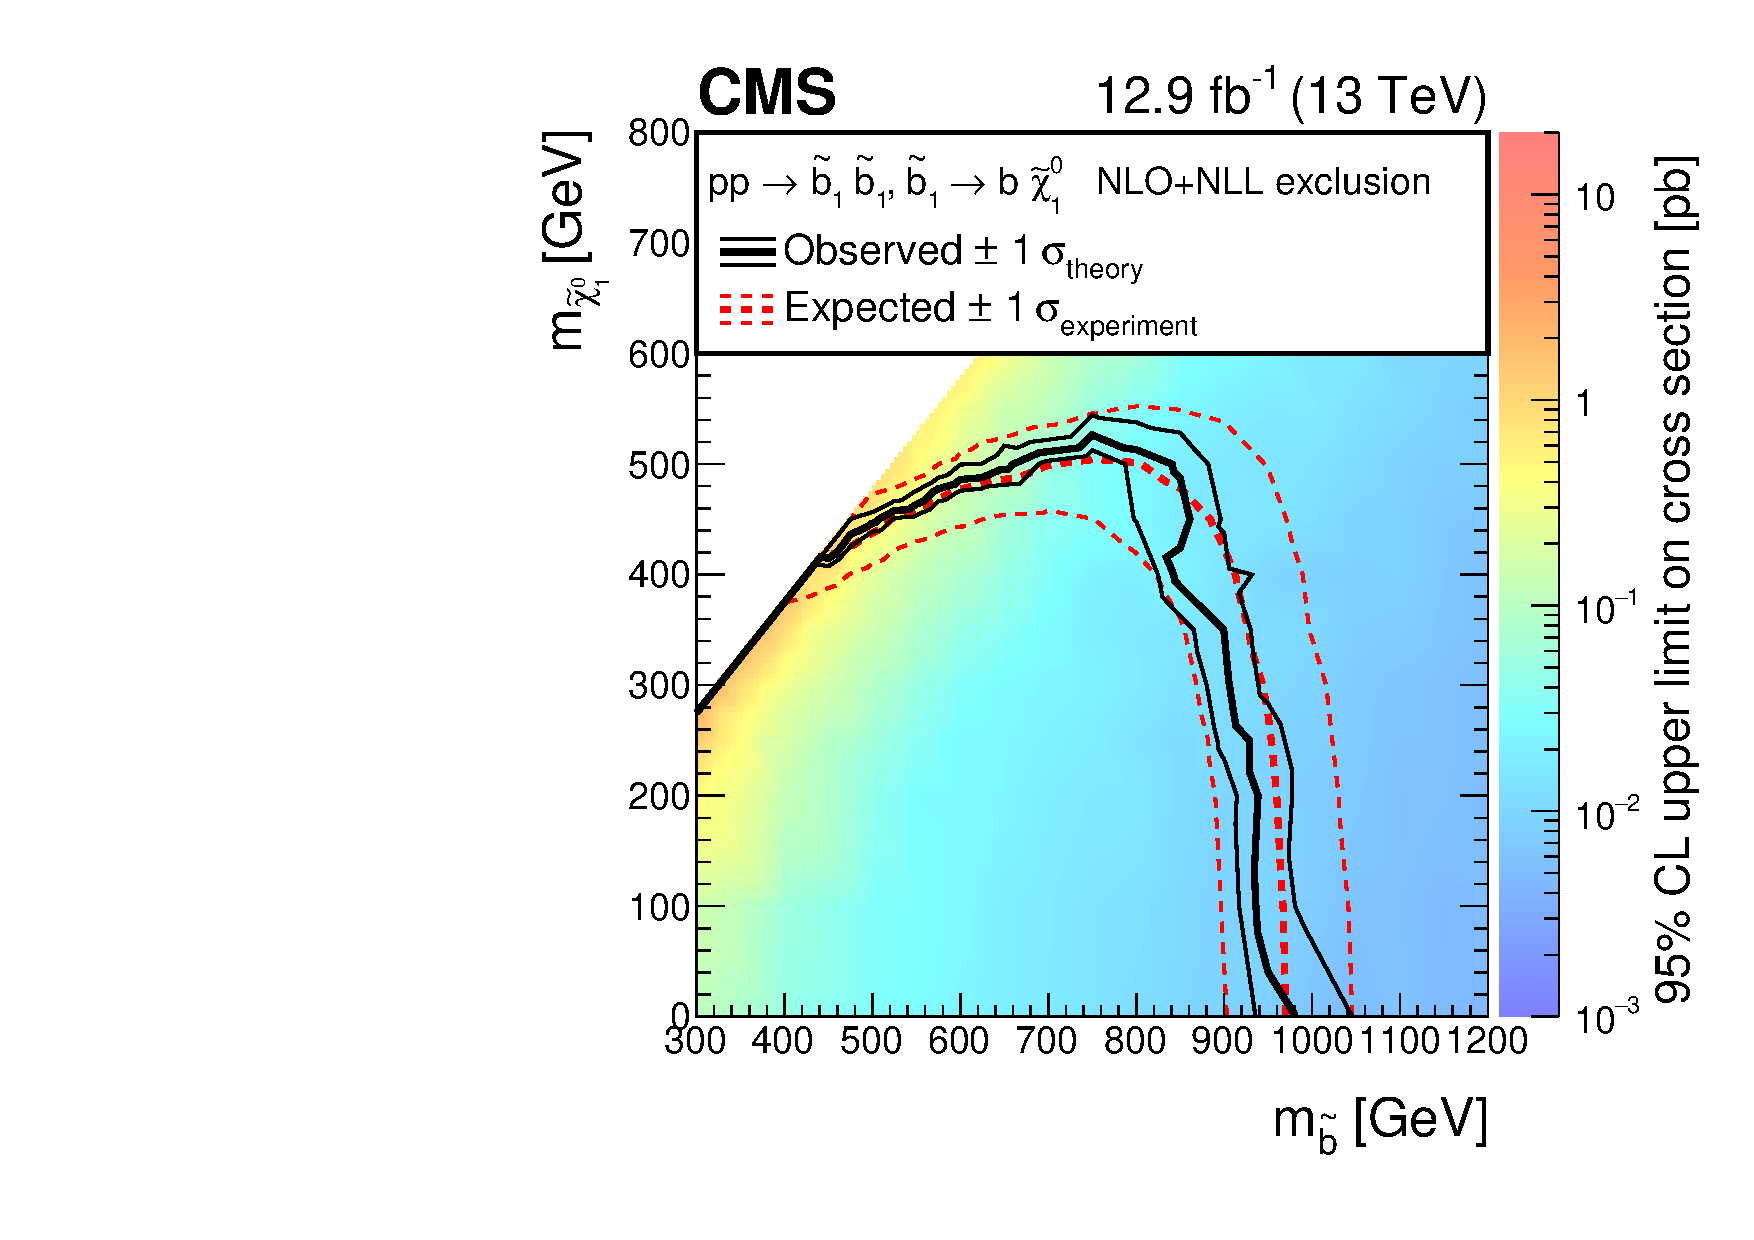
\includegraphics[width=0.49\textwidth]{T2bb.pdf} ~
    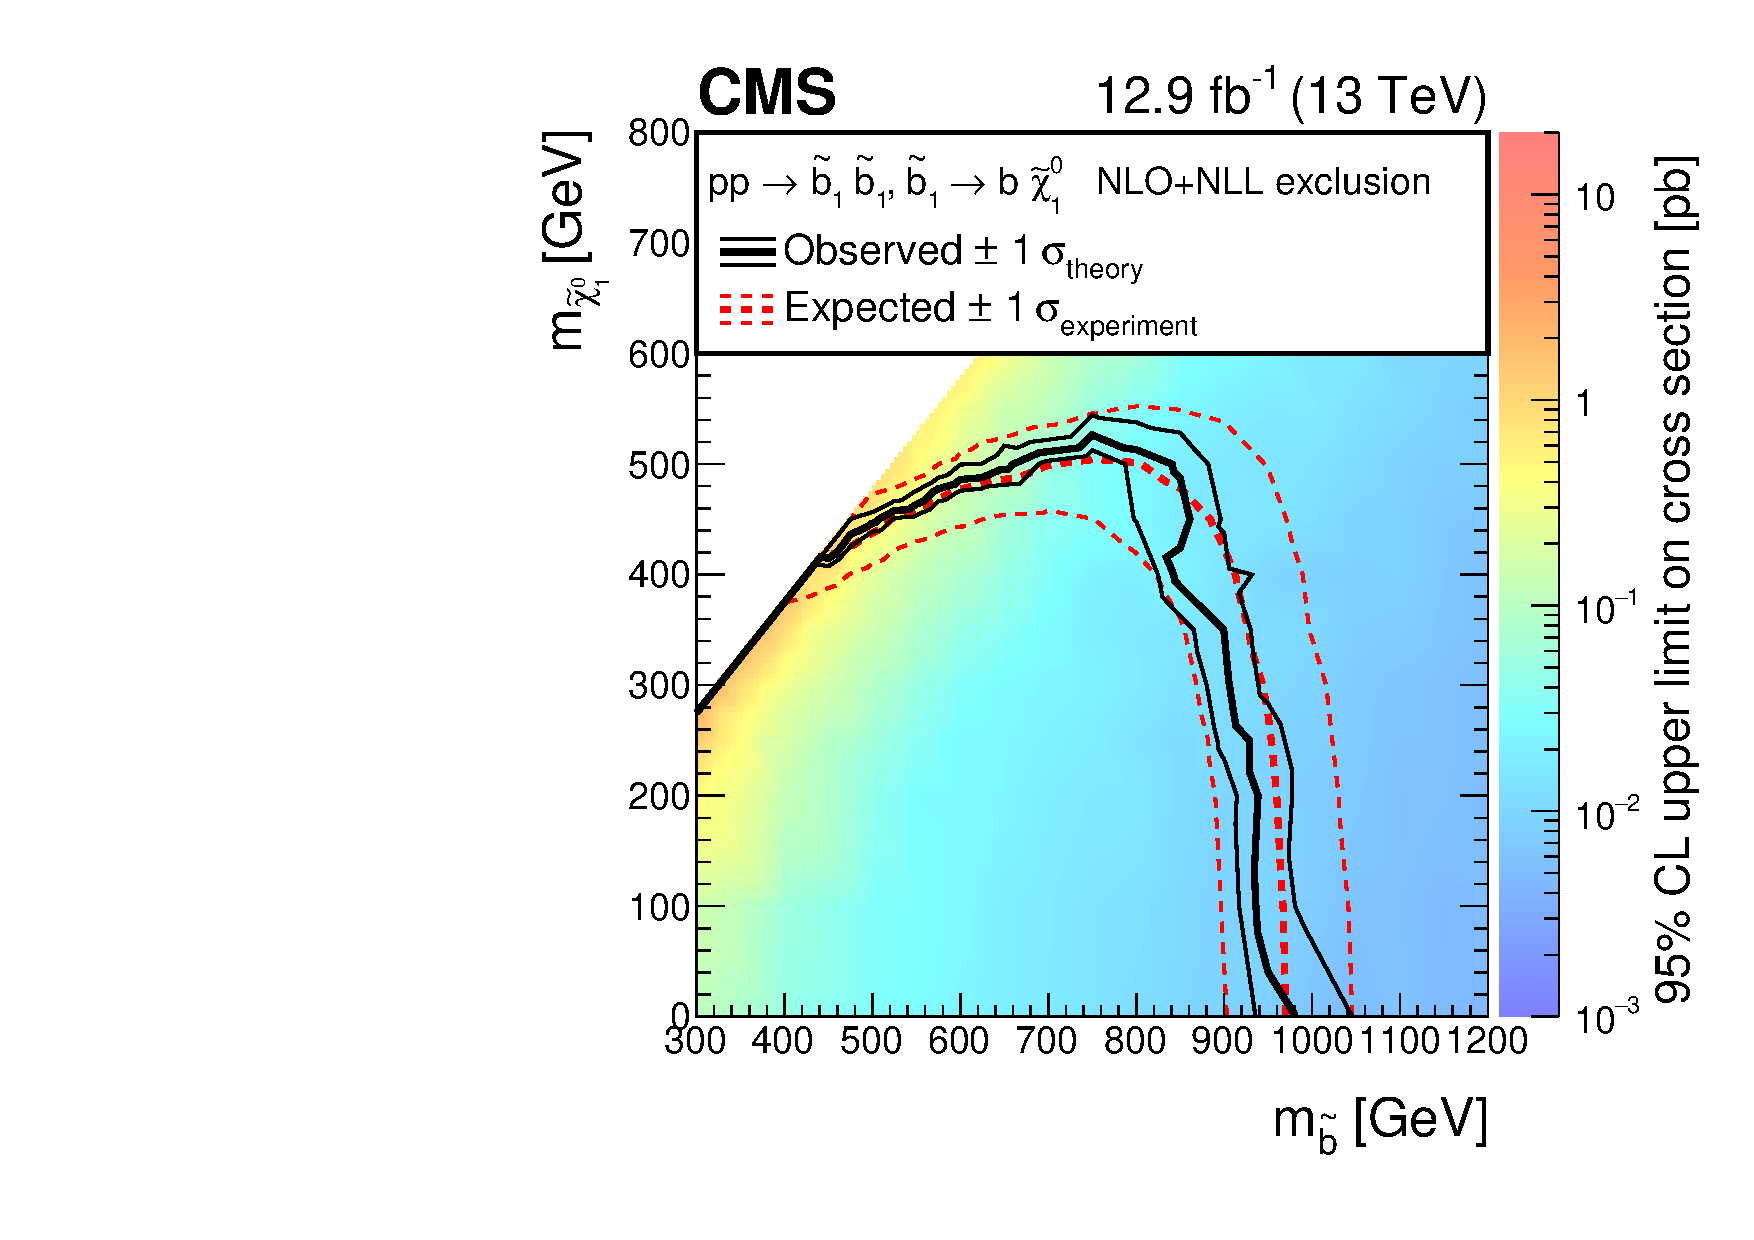
\includegraphics[width=0.49\textwidth]{T2bb.pdf} \\
    \caption{Observed upper limit in cross section at 95\% confidence
      level (indicated by the colour scale) for simplified models that
      assume the gluino-mediated (Left) and direct (Right) production
      of bottom-squark pairs, as a function of, respectively, the
      gluino or bottom squark mass, and the $\chiz_{1}$ mass. The
      black solid thick (thin) line indicates the observed mass
      exclusion regions assuming the nominal (${\pm}1 \sigma$ theory
      uncertainty) production cross section. The red dashed thick
      (thin) line indicates the median (${\pm}1 \sigma$ experimental
      uncertainty) expected mass exclusion regions. {\color{red} To be
        updated. } }
      \label{fig:limits-sms} 
  \end{center}
\end{figure*}

Figure~\ref{fig:limits-sms} shows the observed upper limit on the
production cross section at 95\% confidence level as a function of the
gluino and LSP masses for models that assume the gluino-mediated and
direct production of bottom squark pairs. Also shown are the observed
mass exclusion regions when varying the production cross section by
its theoretical uncertainty, and the expected mass exclusion regions
with the ${\pm}1$ standard-deviation variations. The search places
stringent limits in the mass parameter space, with observed exclusions
in gluino and \chiz masses as high as, respectively, X\gev and
Y\gev. Similarly, in the case of direct squark production, bottom
squark and \chiz masses as high as X\gev and Y\gev are excluded.

%%__________________________________________________________________||
